From the given information, 
\begin{equation}
 \vec n_1=\myvec{2\\-2\\4},
 \vec n_2 =\myvec{3\\-3\\6},
\end{equation}
and 
\begin{align}
    \theta &= \cos^{-1}\brak{{\frac{\vec{n}_1^{T}\vec{n}_2}{\norm{\vec{n_1}}\norm{\vec{n}_2}}}}
    \\
 &= 0\degree
\end{align}
Hence, the given planes are parallel, as can be seen from Fig. \ref{linform/43/c/fig: PARALLEL planes.}
%
\begin{figure}[ht]
    \centering
   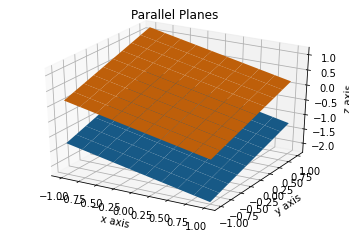
\includegraphics[width=\columnwidth]{solutions/su2021/2/43/c/ASSIGNMENT 5.png}
    \caption{Parallel planes}
    \label{linform/43/c/fig: PARALLEL planes.}
\end{figure}    
